%\documentclass{article}
%\usepackage{graphicx,subfigure}
%\begin{document}

\begin{figure}[h]
  \centering
  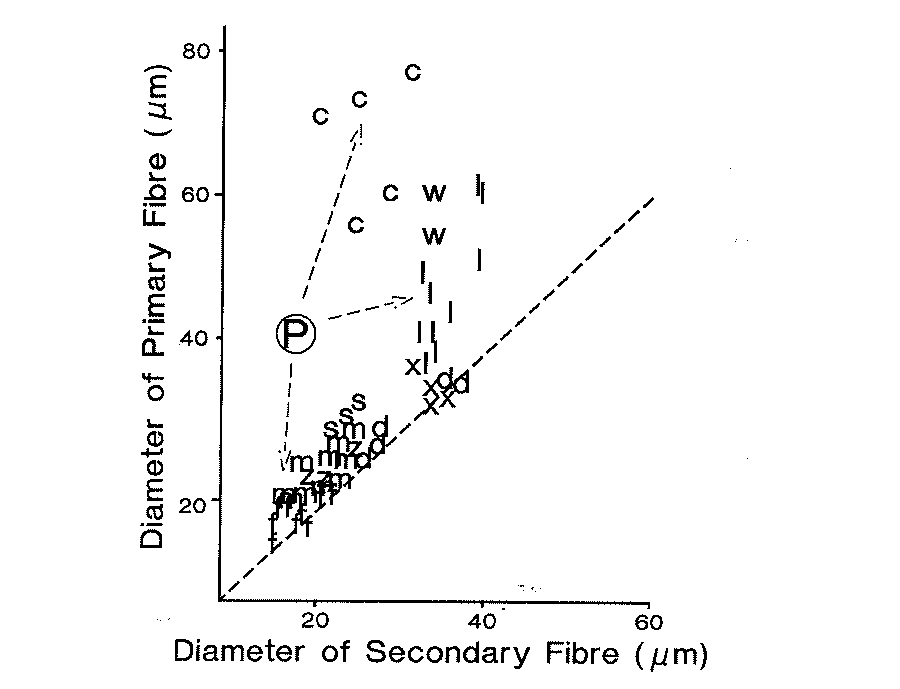
\includegraphics[width=1.3\textwidth, trim = 80 0 0 120]{images/fig5.png}
  \caption{   Relationship of primary fibre diameter (Dp) to secondary fibre
	      diameter (Ds) across a range of breeds.  Data from Carter (1968)
	  and CSIRO (unpublished).  Suggested lines of evolution of the
          major breeds shown $-\ -\ -\ -\ ->$.  $Dp/Ds$ ratio $ = 1$ 
	  shown $-\ -\ -\ -\ -\ -$. Letter codes denote breed;
f,  Fine Merino;
m,  Medium Merino;
s,  Strong Merino;
z,  Polwarth;
x,  Corriedale;
l,  Longwool;
d,  Downwool;
c,  Carpet Wool;
P,  Primitive;
w,  Wiltshire Horn. }
  \label{fig:5}
\end{figure}

%\end{document}
